\documentclass[12pt]{beamer}

% Theme & Colors
\usetheme{Madrid} % Try: Berlin, Copenhagen, CambridgeUS, Warsaw...
\usecolortheme{dolphin} % Try: seahorse, crane, beaver...

% Encoding & Fonts
\usepackage[utf8]{inputenc}
\usepackage[T1]{fontenc}
\usepackage{lmodern} % Better font
\usepackage{luatexja}
\usepackage{luatexja-fontspec}
\usepackage{amsmath,amssymb,mathtools,ascmac,amsthm,amscd,tikz-cd}
\usetikzlibrary{arrows.meta,calc,quotes,angles}
\setmainjfont{Noto Sans CJK JP}

% Title Information
\newcommand{\circnum}[2][]{%
  \tikz[baseline=(n.base)] \node (n) [circnum,#1]{#2};%
}
\title[]{円の性質}
\date{\today}

\begin{document}
% Title Page
\begin{frame}
  \titlepage
\end{frame}

% Outline
\begin{frame}{}
  \tableofcontents
\end{frame}

% Section 1
\section{円周角の定理とその逆}
\begin{frame}{}
  \begin{block}{定理10. 円周角の定理 (Inscribed angle theorem)}
		1つの弧に対する円周角の大きさは一定であり,その弧に対する中心角の大きさの半分である.
  \end{block}
	\begin{center}
		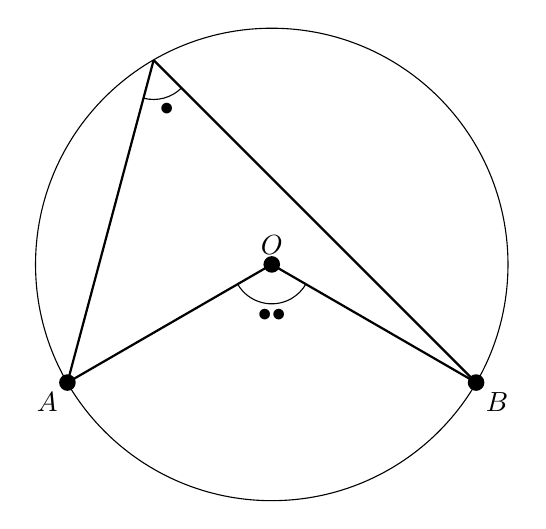
\begin{tikzpicture}[scale=3]
  % Define the vertices
  \coordinate (O) at (0,0);
  \coordinate (A) at (-0.865,-1/2);
  \coordinate (B) at (0.865,-1/2);
  \coordinate (C) at (-1/2,0.865);
	 \draw (O) circle (1);
  % Draw the triangle
	\draw[thick] (A)--(C);
	\draw[thick] (B)--(C);
	\draw[thick] (A)--(O);
	\draw[thick] (B)--(O);
  \fill (O) circle (1pt) node[above] {$O$};
  \fill (A) circle (1pt) node[below left] {$A$};
  \fill (B) circle (1pt) node[below right] {$B$};
	 \path pic["$\bullet $",draw,angle radius=5mm,angle eccentricity=1.3] {angle = A--C--B};
	 \path pic["$\bullet \bullet$",draw,angle radius=5mm,angle eccentricity=1.3] {angle = A--O--B};
\end{tikzpicture}
\end{center}
\end{frame}

\begin{frame}{}
  \begin{block}{定理11.\\ 円周角の定理の逆 (Converse inscribed angle theorem)}
		$P,	Q$が直線$A,B$に関して同じ側にあるとき,
\[\angle APB = \angle AQB.\]
ならば,4点$A,B,P,Q$は同一円周上にある.
  \end{block}
\begin{center}
		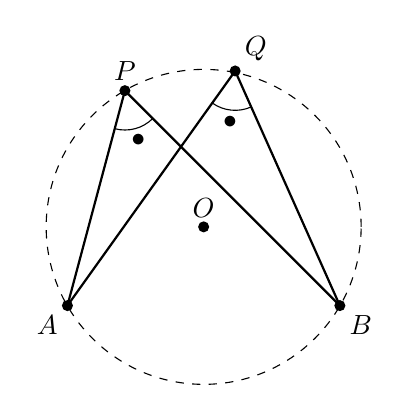
\begin{tikzpicture}[scale=2]
  % Define the vertices
  \coordinate (O) at (0,0);
  \coordinate (A) at (-0.865,-1/2);
  \coordinate (B) at (0.865,-1/2);
  \coordinate (P) at (-1/2,0.865);
  \coordinate (Q) at (0.2,0.99);
	\draw[dashed] (O) circle (1);
  % Draw the triangle
	\draw[thick] (A)--(P)--(B);
	%\draw[thick] (A)--(O)--(B);
	\draw[thick] (A)--(Q)--(B);
  \fill (O) circle (1pt) node[above] {$O$};
  \fill (A) circle (1pt) node[below left] {$A$};
  \fill (B) circle (1pt) node[below right] {$B$};
  \fill (P) circle (1pt) node[above] {$P$};
  \fill (Q) circle (1pt) node[above right] {$Q$};
	 \path pic["$\bullet $",draw,angle radius=5mm,angle eccentricity=1.3] {angle = A--P--B};
	 \path pic["$\bullet $",draw,angle radius=5mm,angle eccentricity=1.3] {angle = A--Q--B};
\end{tikzpicture}
\end{center}
\end{frame}

\section{円に内接する四角形}
\begin{frame}{円に内接する四角形}
	\begin{block}{定義}
		四角形の4つの頂点すべてを通る円があるとき,この四角形は円に\textbf{内接する}という.
	\end{block}
\begin{center}
		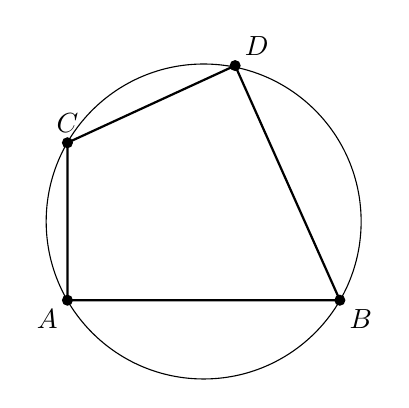
\begin{tikzpicture}[scale=2]
  % Define the vertices
  \coordinate (O) at (0,0);
  \coordinate (A) at (-0.865,-1/2);
  \coordinate (B) at (0.865,-1/2);
  \coordinate (P) at (-0.865,0.5);
  \coordinate (Q) at (0.2,0.99);
	\draw[] (O) circle (1);
  % Draw the triangle
	%\draw[thick] (A)--(O)--(B);
	\draw[thick] (A)--(B)--(Q)--(P)--cycle;
  %\fill (O) circle (1pt) node[above] {$O$};
  \fill (A) circle (1pt) node[below left] {$A$};
  \fill (B) circle (1pt) node[below right] {$B$};
  \fill (P) circle (1pt) node[above] {$C$};
  \fill (Q) circle (1pt) node[above right] {$D$};
%	 \path pic["$\bullet $",draw,angle radius=5mm,angle eccentricity=1.3] {angle = A--P--B};
%	 \path pic["$\bullet $",draw,angle radius=5mm,angle eccentricity=1.3] {angle = A--Q--B};
\end{tikzpicture}
\end{center}
$\longrightarrow$三角形は円に内接するが,四角形は必ずしも内接するとは限らない.
\end{frame}

\begin{frame}{円に内接する四角形}
	\begin{block}{定理12. 円に内接する四角形の内角\cdot 外角}
		四角形に円が内接するとき,次の(1), (2)がなりたつ.
		\begin{itemize}
			\item [(1)]
				向かい合う内角の和は$180^\circ$である.
			\item [(2)]
				内角は,それに向かい合う角の外角に等しい.
		\end{itemize}
	\end{block}
\begin{center}
		\begin{tikzpicture}[scale=2]
  % Define the vertices
  \coordinate (O) at (0,0);
  \coordinate (A) at (-0.865,-1/2);
  \coordinate (B) at (0.865,-1/2);
  \coordinate (B') at (2,-1/2);
  \coordinate (C) at (-0.865,0.5);
  \coordinate (D) at (0.2,0.99);
	\draw[] (O) circle (1);
  % Draw the triangle
	%\draw[thick] (A)--(O)--(B);
	\draw[thick] (A)--(B)--(Q)--(P)--cycle;
	\draw[thick] (B)--(B');
  %\fill (O) circle (1pt) node[above] {$O$};
  \fill (A) circle (1pt) node[below left] {$A$};
  \fill (B) circle (1pt) node[below right] {$B$};
  \fill (C) circle (1pt) node[above] {$C$};
  \fill (D) circle (1pt) node[above right] {$D$};
	 \path pic["$\bullet $",draw,angle radius=5mm,angle eccentricity=1.3] {angle = A--C--D};
	 \path pic["$\circ $",draw,angle radius=5mm,angle eccentricity=1.3] {angle = D--B--A};
	 \path pic["$\bullet $",draw,angle radius=7mm,angle eccentricity=1.3] {angle = B'--B--D};
\end{tikzpicture}
\end{center}
\end{frame}

\end{document}
